% Filename: Results
% Last update: Monday, 12/9/2018 by Ally Warner
%
%%%%%%%%%%%%%%%%%%%%%%%%%%%%%%%%%%%%%%%%%%%%%%%%%%%%%%%%%%%%%%%%%%%%%%

\section{Results}
\label{sec:results}

All SCIRun networks used to generate results are included in an open-source dataset for research use at \url{www.sci.utah.edu/SCI_headmodel}.

\subsection{Segmentation}

For this project, we segmented the head into eight detailed layers listed in Section \ref{sec:Seg}. We used this mesh to create an inhomogeneous three-dimensional tetrahedral mesh.

\begin{figure}[H]
\begin{center}
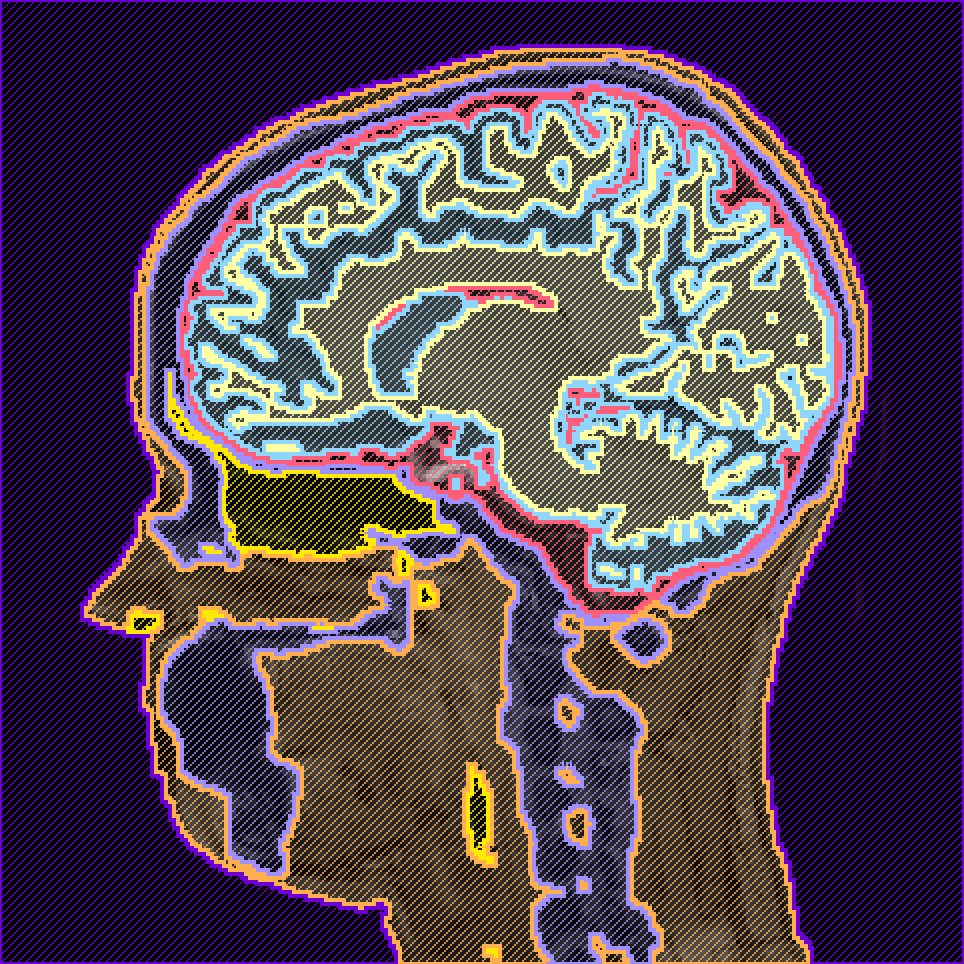
\includegraphics[height=2.35in]{Figures/seg_1}
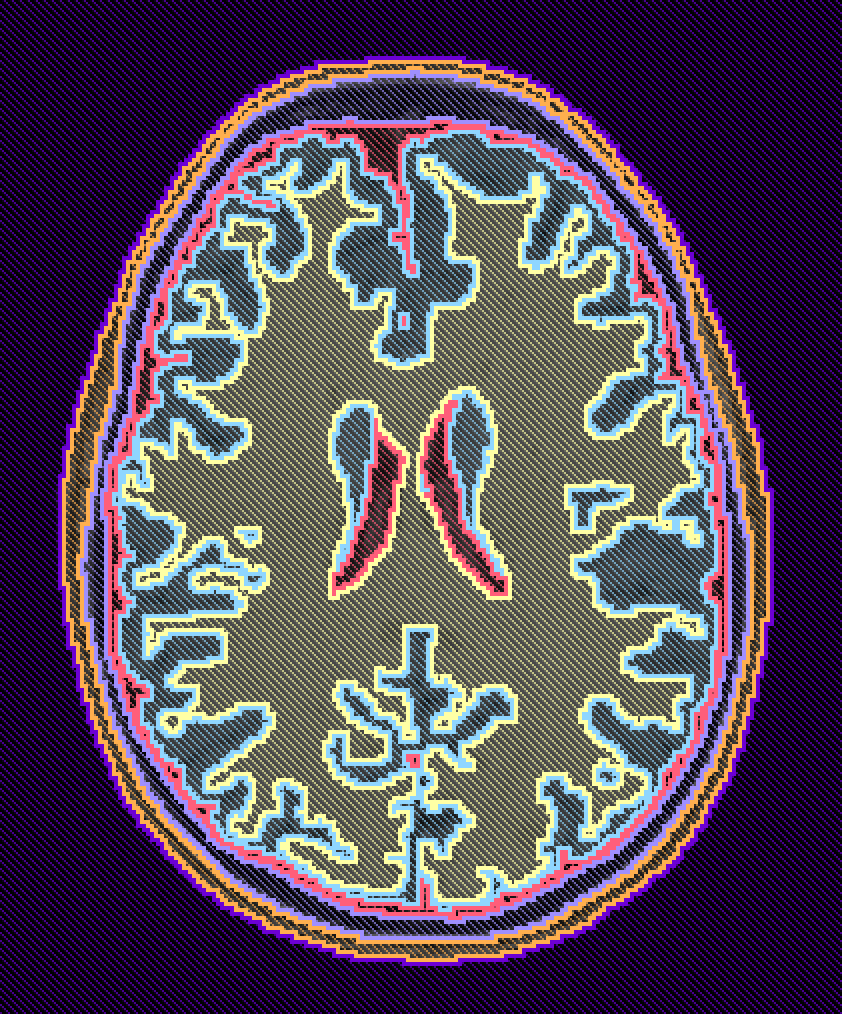
\includegraphics[height=2.35in]{Figures/seg_2}
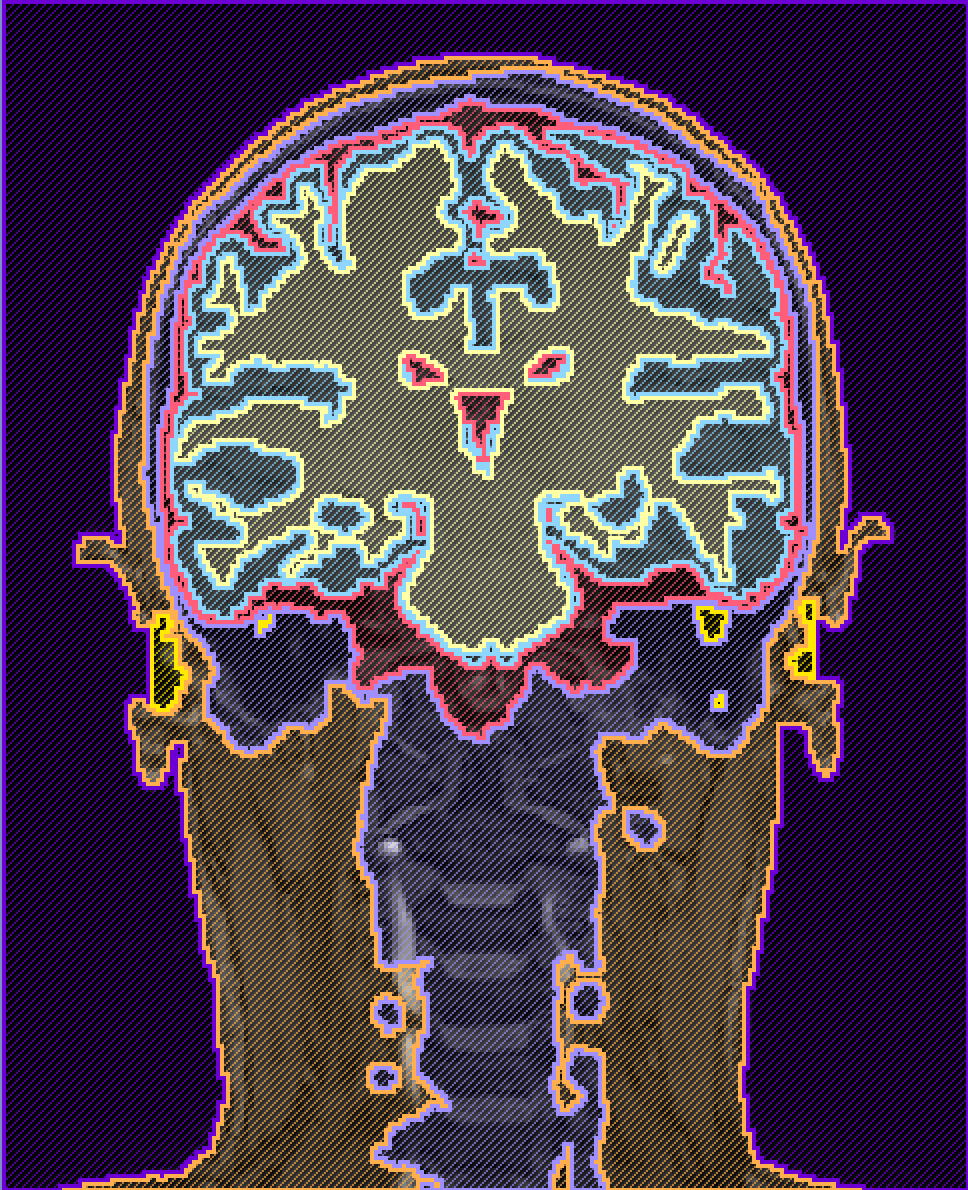
\includegraphics[height=2.35in]{Figures/seg_3}
\caption{A high-resolution, eight-layer, full head segmentation made with Seg3D}
\label{fig:fullseg}
\end{center}
\end{figure}

Since the dataset did not include a CT scan, the task of segmenting the skull and the sinus layers were the most challenging. As described in Section \ref{sec:Seg}, our first attempt at a bone segmentation was to combine a skull made from FSL \cite{ref:bet2} with bones thresholded using Seg3D. Although we had a bone segmentation, the sinus segmentation was not completed from this segmentation since it would have to be created manually.

The skull/bone and sinus segmentations we made from the pseudo-CT scan were smooth and connected segmentations and fit well into the entire head segmentation.

\begin{figure}[H]
\begin{center}
\includegraphics[width=.49\textwidth]{Figures/skull_before}
\includegraphics[width=.49\textwidth]{Figures/skull_after}
\caption{Skull segmentation comparison: Created with BET and thresholding \textit{(left)} and with pseudo-CT \textit{(right)}. Both segmentations were made using Seg3D}
\label{fig:skull}
\end{center}
\end{figure}

\begin{figure}[H]
\begin{center}
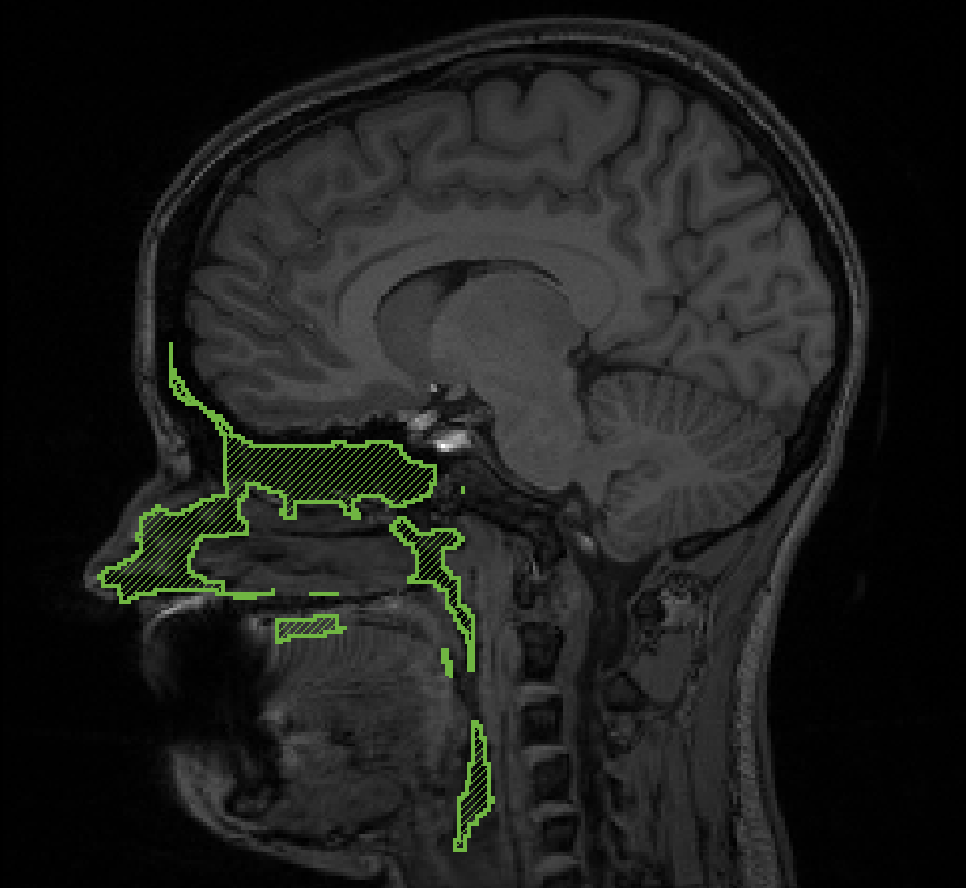
\includegraphics[width=.49\textwidth]{Figures/sinus_sag}
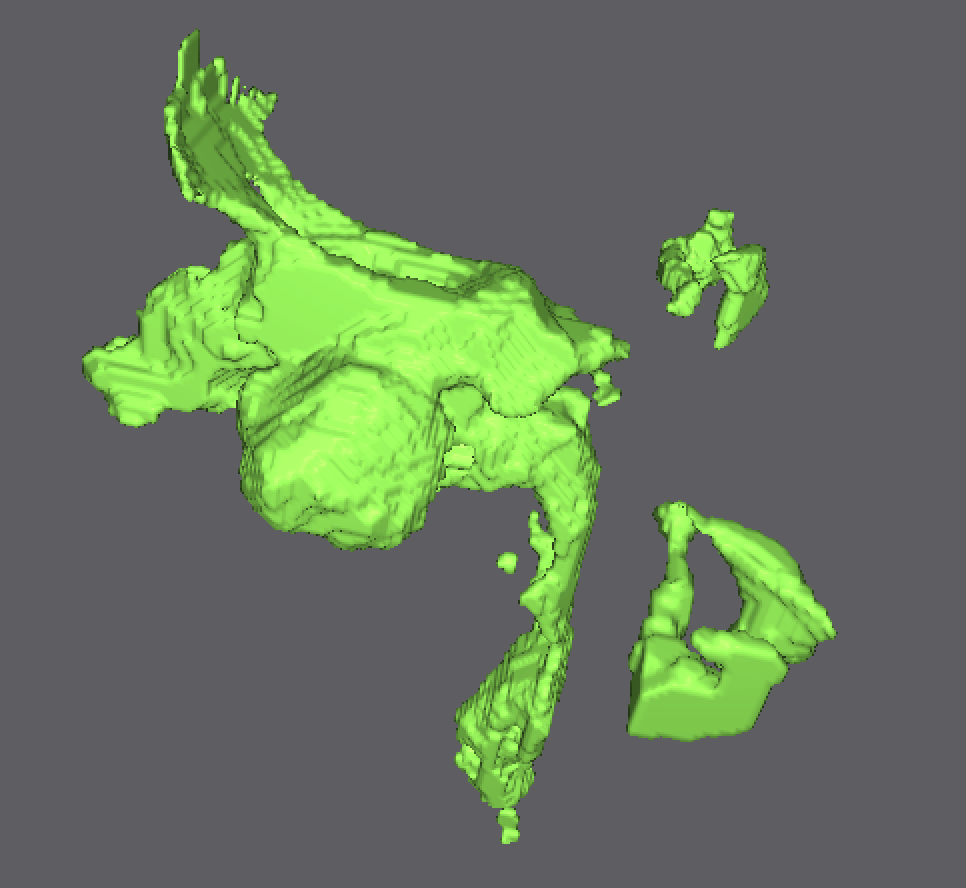
\includegraphics[width=.49\textwidth]{Figures/sinus_iso}
\caption{Sinus segmentation}
\label{fig:sinus}
\end{center}
\end{figure}

During MRI imaging, the subject was on her back, which caused the brain to shift to the back of the head, resulting in thin segmented sections on the back of the head as well as on the side of the subject's head, the bridge of the nose, and the bottom of the chin. We made these sections at least two pixels thick to ensure a mesh without holes.

\begin{figure}[H]
\begin{center}
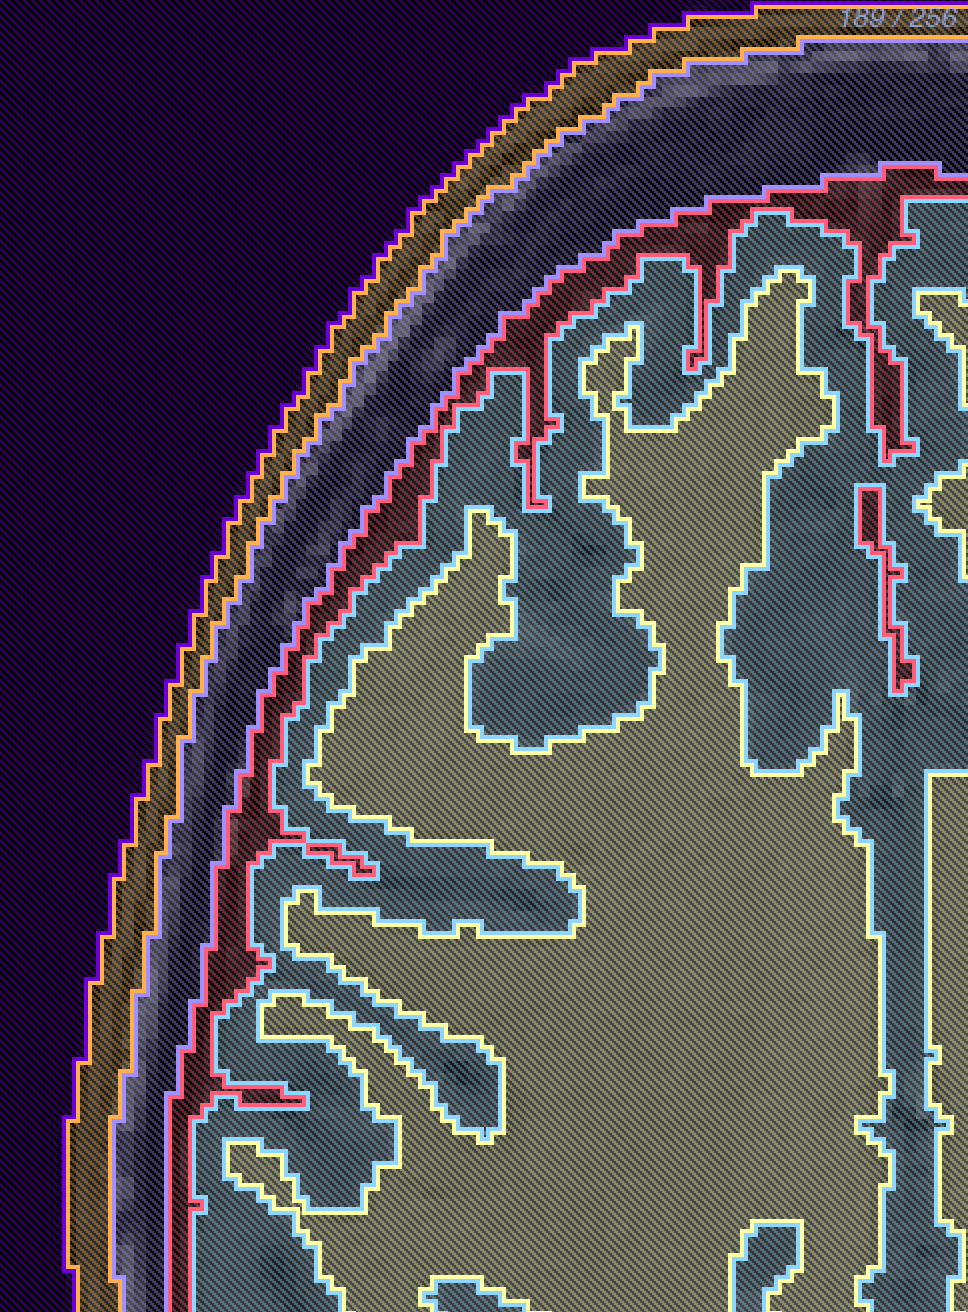
\includegraphics[width=.32\textwidth]{Figures/thin_layer_side}
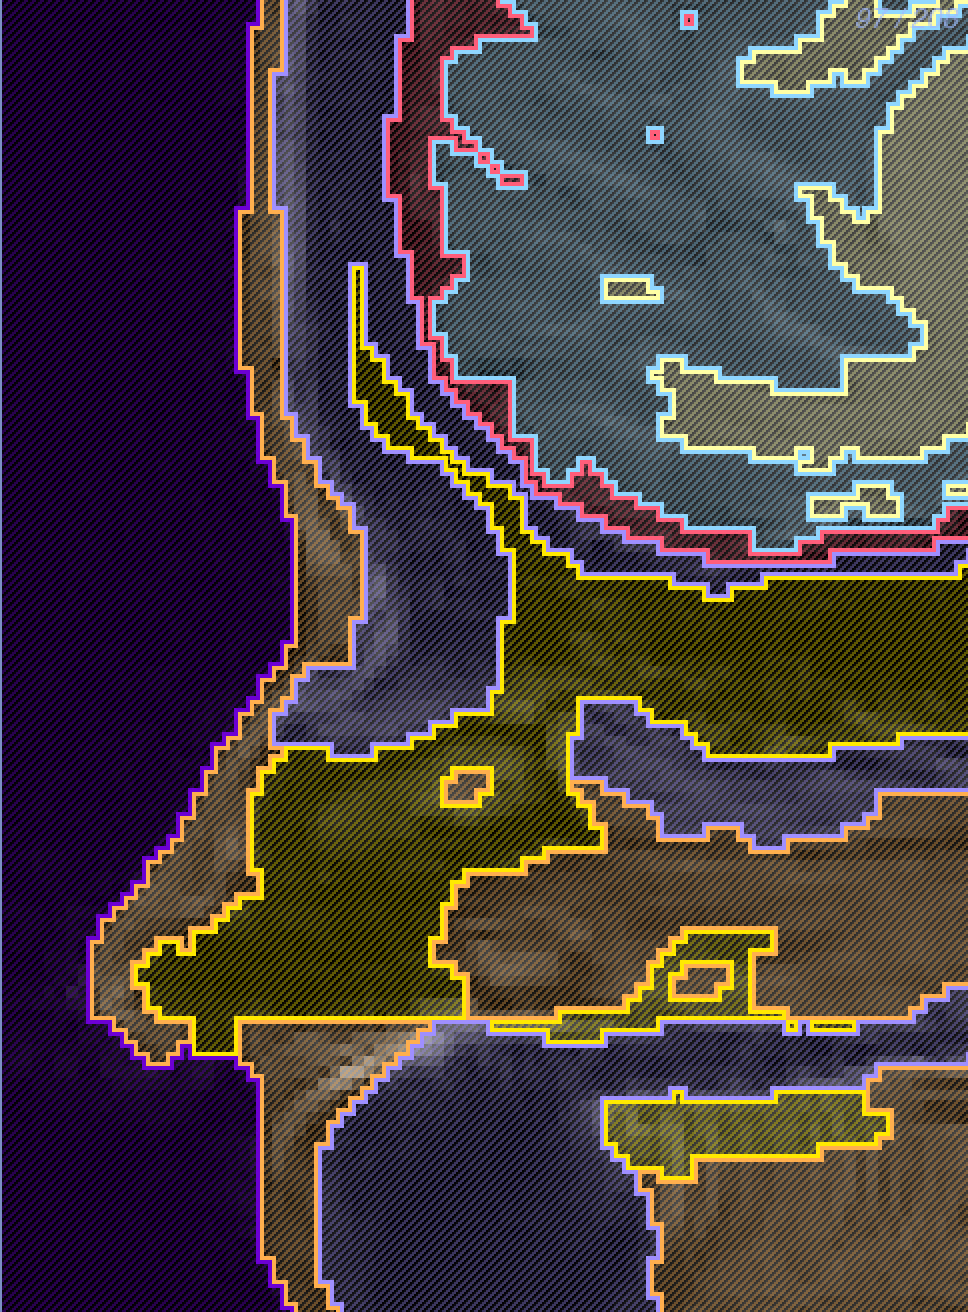
\includegraphics[width=.32\textwidth]{Figures/thin_layer_nose}
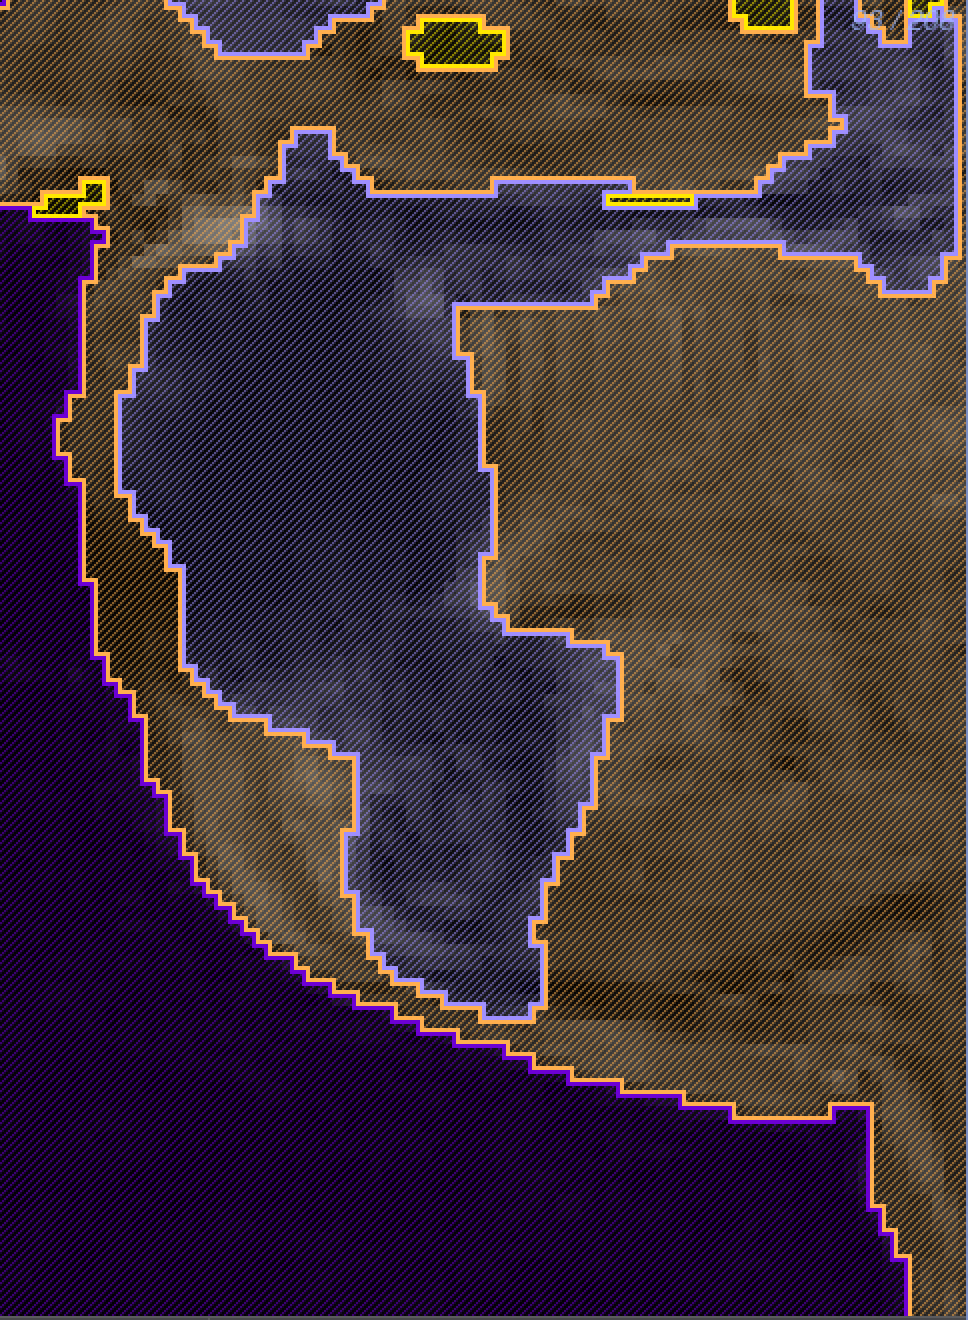
\includegraphics[width=.32\textwidth]{Figures/thin_layer_chin}
\caption{Thin segmentation sections: side of the head \textit{(left)}, bridge of the nose \textit{(middle)}, bottom of the chin \textit{(right)}}
\label{fig:thinseg}
\end{center}
\end{figure}

\subsection{Finite Element Meshes}

The highest resolution mesh we generated with the settings listed in Section \ref{sec:mesh} had 60.2 million elements and 10.3 million nodes. This mesh was large because of the complexity of the segmentation, including small features, thin sections, and several layers touching at once. The simulations performed slowly when using this mesh due to its size and required at least 32GB of RAM.

\begin{figure}[H]
\begin{center}
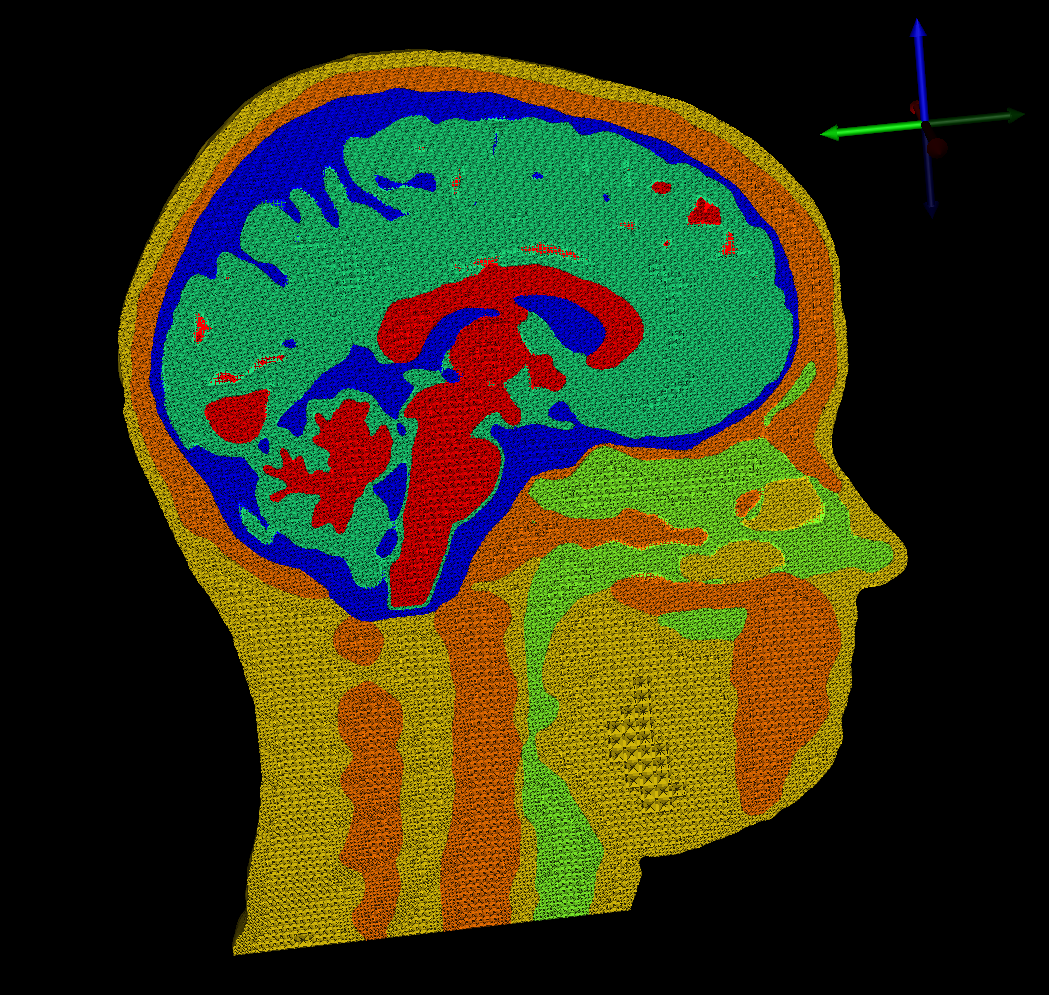
\includegraphics[width=.49\textwidth]{Figures/bigmesh_1}
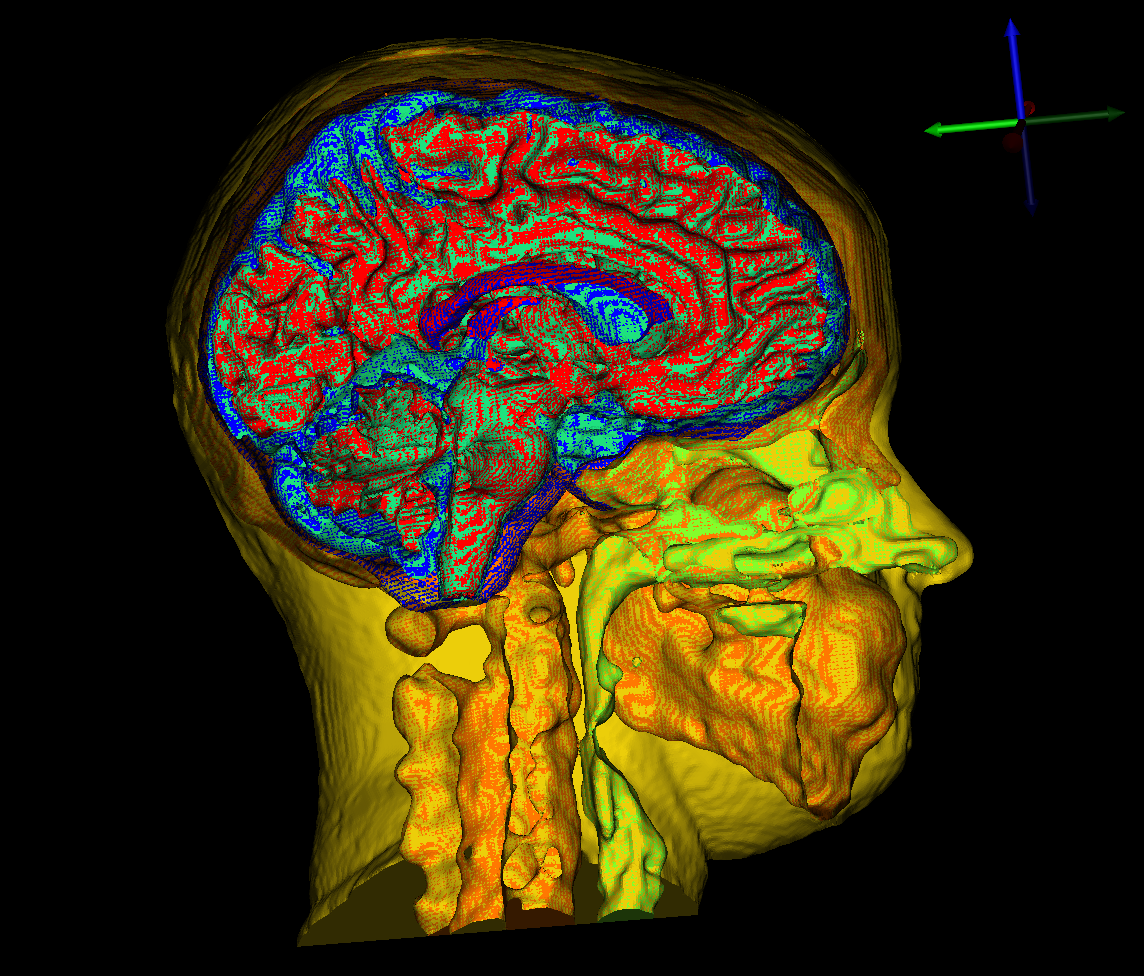
\includegraphics[width=.49\textwidth]{Figures/bigmesh_surface}
\caption{60.2 M element mesh: tetrahedral mesh \textit{(left)}, surface mesh \textit{(right)}}
\label{fig:bigmesh}
\end{center}
\end{figure}

We attempted to generate smaller meshes to be able to run quicker simulations, but many of the meshes contained holes. After we manually changed the sizing field described in Section \ref{sec:mesh}, we generated a mesh with 15.7 million elements and 2.7 million nodes without holes. However, this mesh contained one flat tetrahedra, which we later removed in a SCIRun network. This issue is currently being investigated by Cleaver software developers.

\begin{figure}[H]
\begin{center}
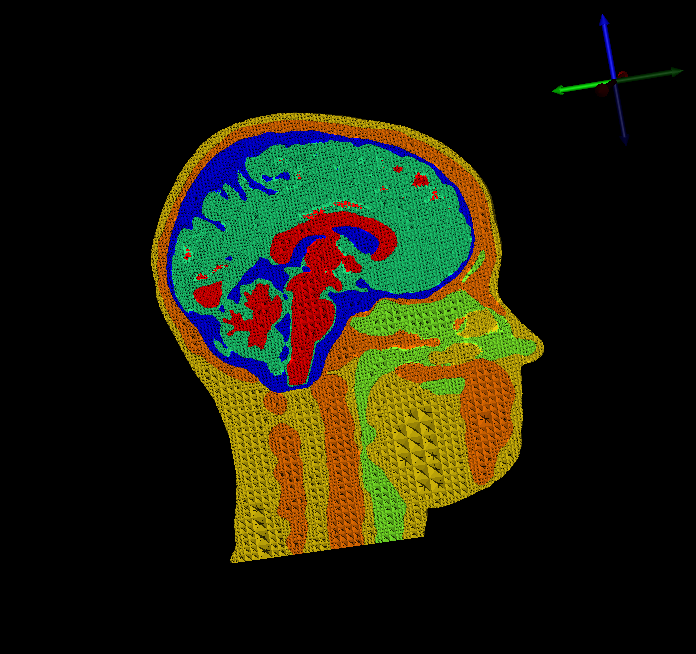
\includegraphics[width=.49\textwidth]{Figures/smallmesh_2}
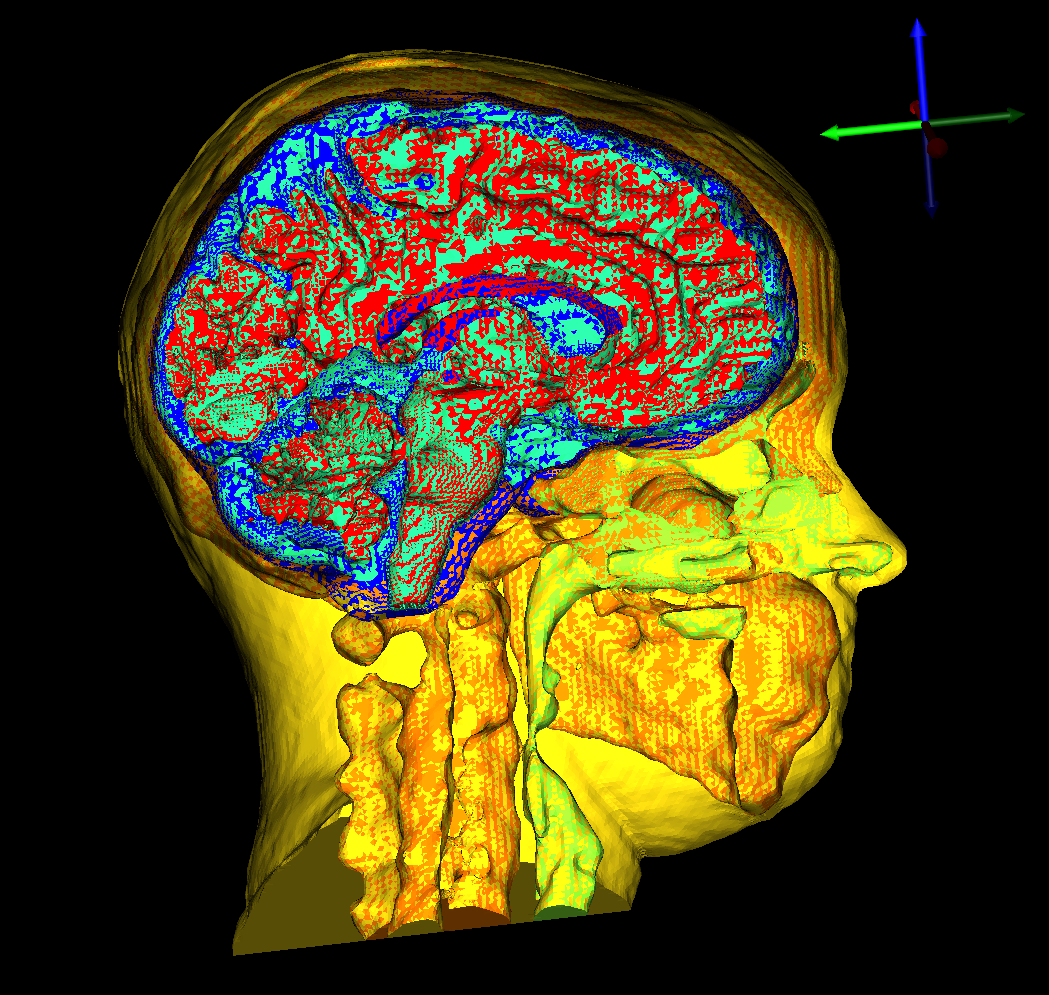
\includegraphics[width=.49\textwidth]{Figures/smallmesh_surface}
\caption{15.7 M element mesh: tetrahedral mesh \textit{(left)}, surface mesh \textit{(right)}}
\label{fig:smallmesh}
\end{center}
\end{figure}

\subsection{Forward Problem}

\subsubsection{Isotropic}

An isotropic, inhomogeneous head model is expected to have largely spherical propagation of electrical signals. We generated three-dimensional streamlines, as well as, isolines to visualize this propagation and to compare isotropic and anisotropic conductivity. The simulations showed spherical propagation and acceptable registration of electrodes and dipoles to the mesh space.

\begin{figure}[H]
\begin{center}
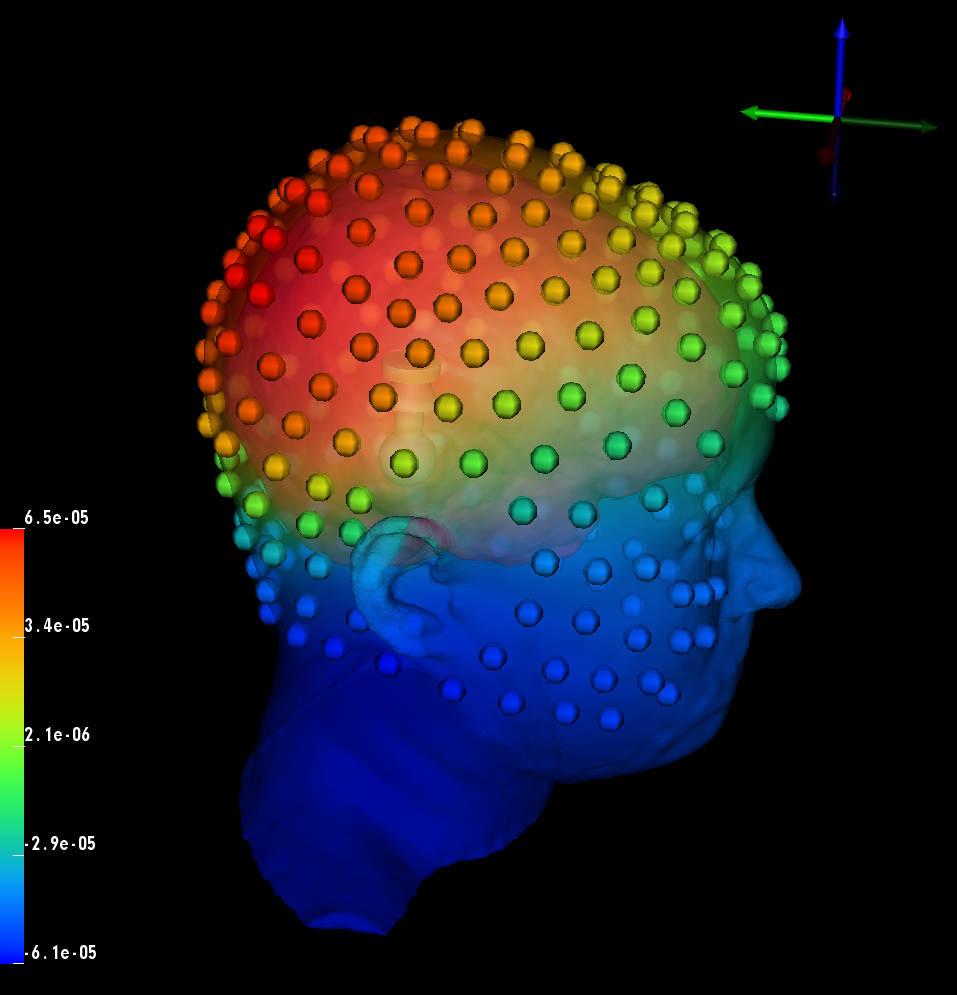
\includegraphics[width=.49\textwidth]{Figures/iso_dipole}
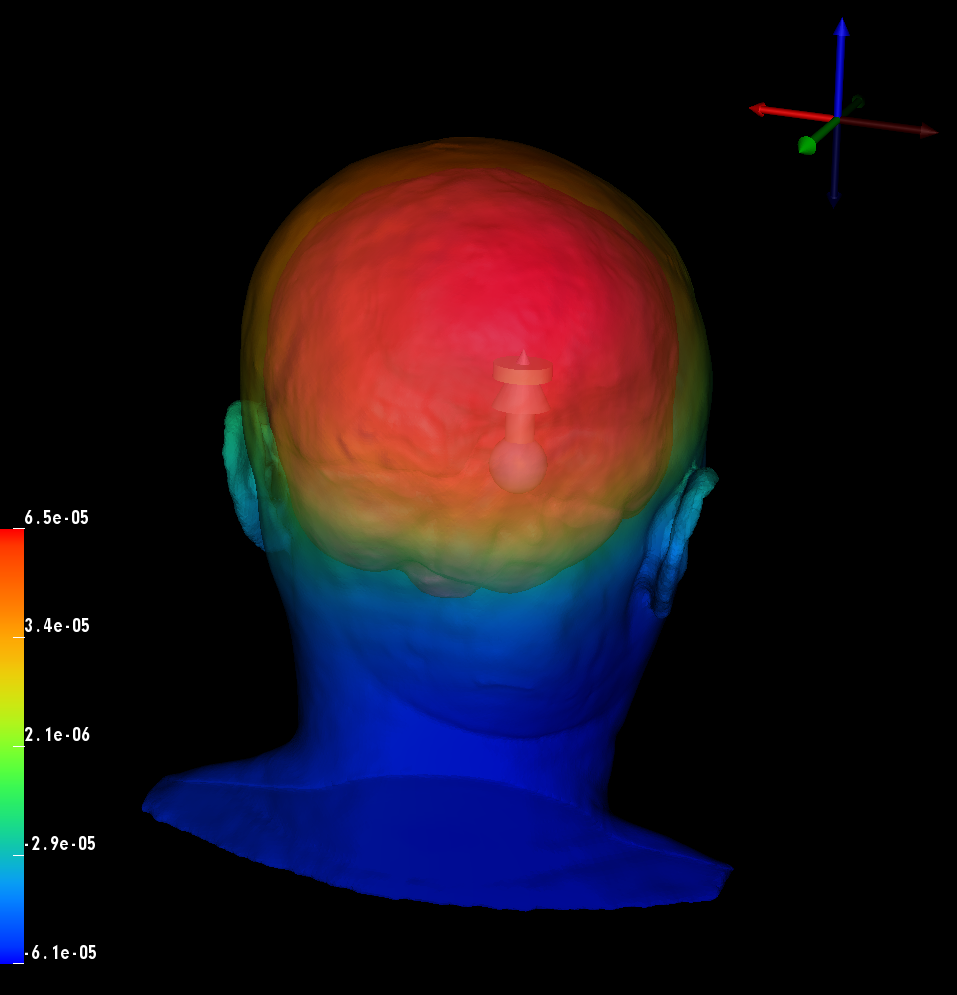
\includegraphics[width=.49\textwidth]{Figures/iso_dipole_2}
\caption{Isotropic forward problem solution with dipole source and data mapped onto the head surface and electrodes}
\label{fig:isodip}
\end{center}
\end{figure}

\begin{figure}[H]
\begin{center}
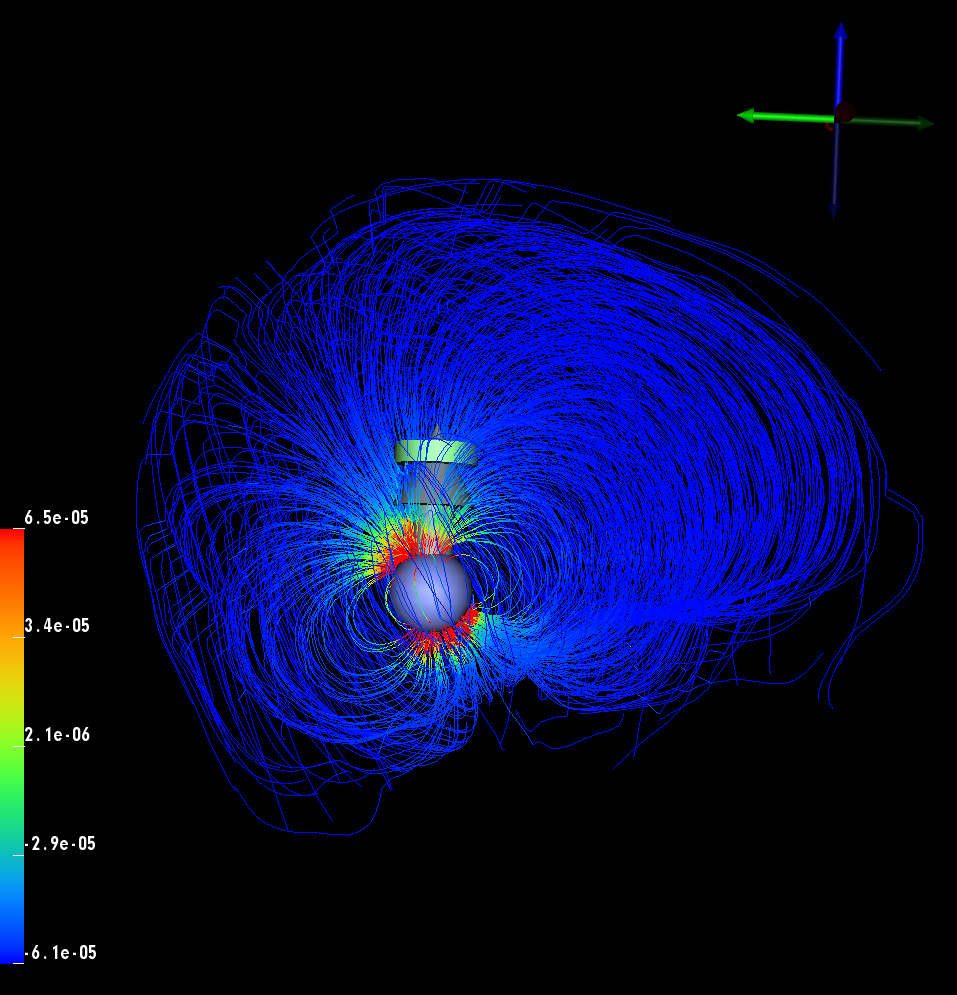
\includegraphics[width=.49\textwidth]{Figures/iso_streamlines}
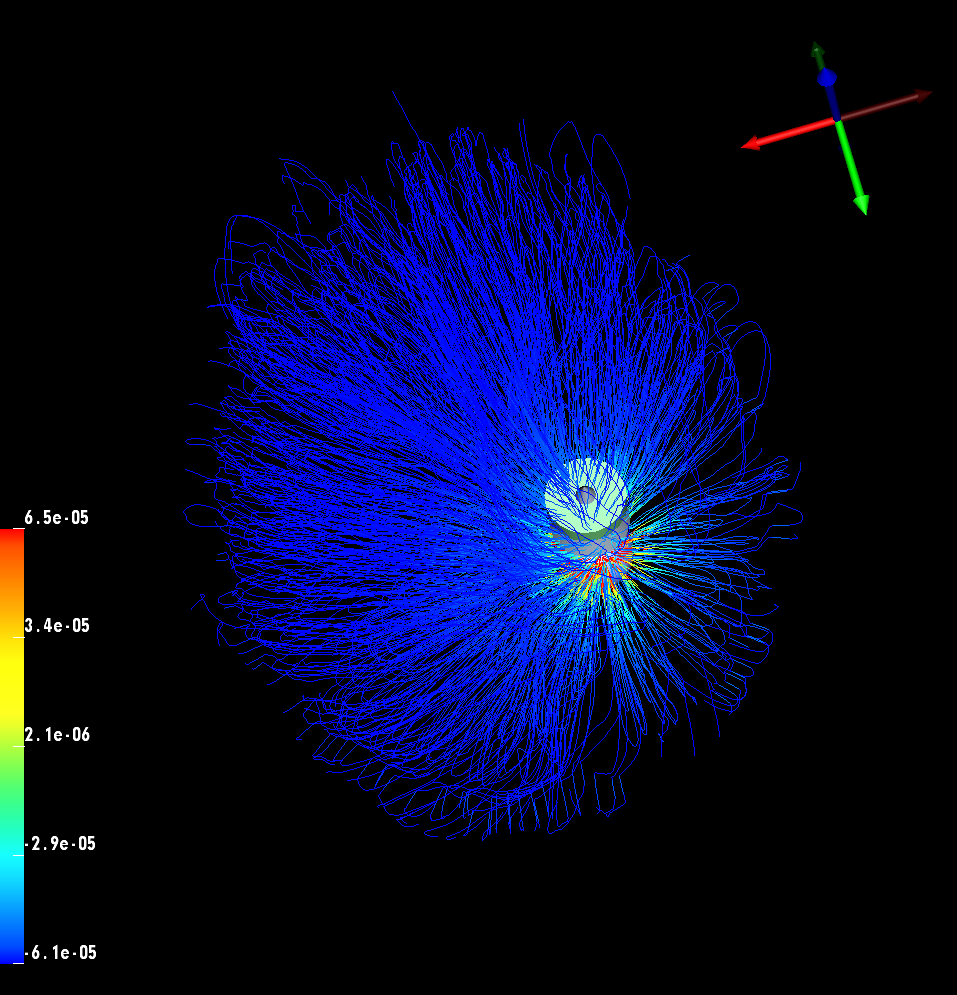
\includegraphics[width=.49\textwidth]{Figures/iso_streamlines_top}
\caption{Isotropic streamlines with dipole source}
\label{fig:isostream}
\end{center}
\end{figure}

\subsubsection{Anisotropic}

The expectation for an anisotropic, inhomogeneous head model is to have nonspherical propagation, which can be seen with the streamlines and isolines visualizations. As discussed in Section \ref{sec:cond}, two methods are used for scaling diffusion tensor data. We built the SCIRun network with the option to choose either scaling method. The simulations showed nonspherical propagation and acceptable registration of the electrodes, dipoles, and mesh into the diffusion tensor space.

\begin{figure}[H]
\begin{center}
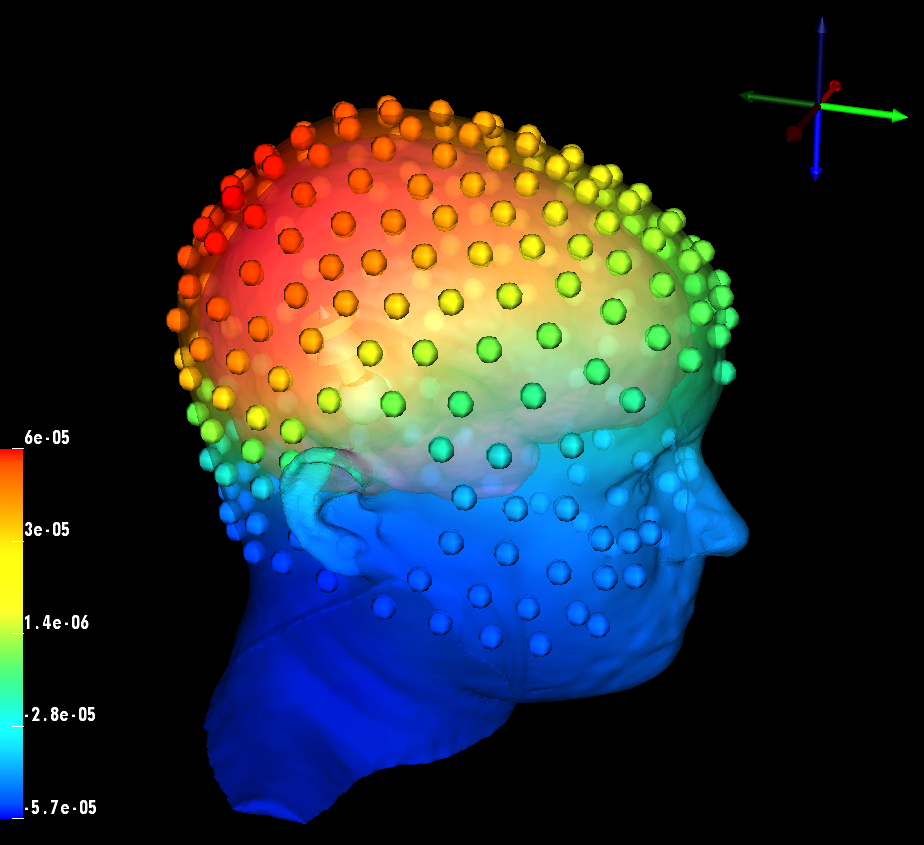
\includegraphics[width=.49\textwidth]{Figures/aniso_dipole}
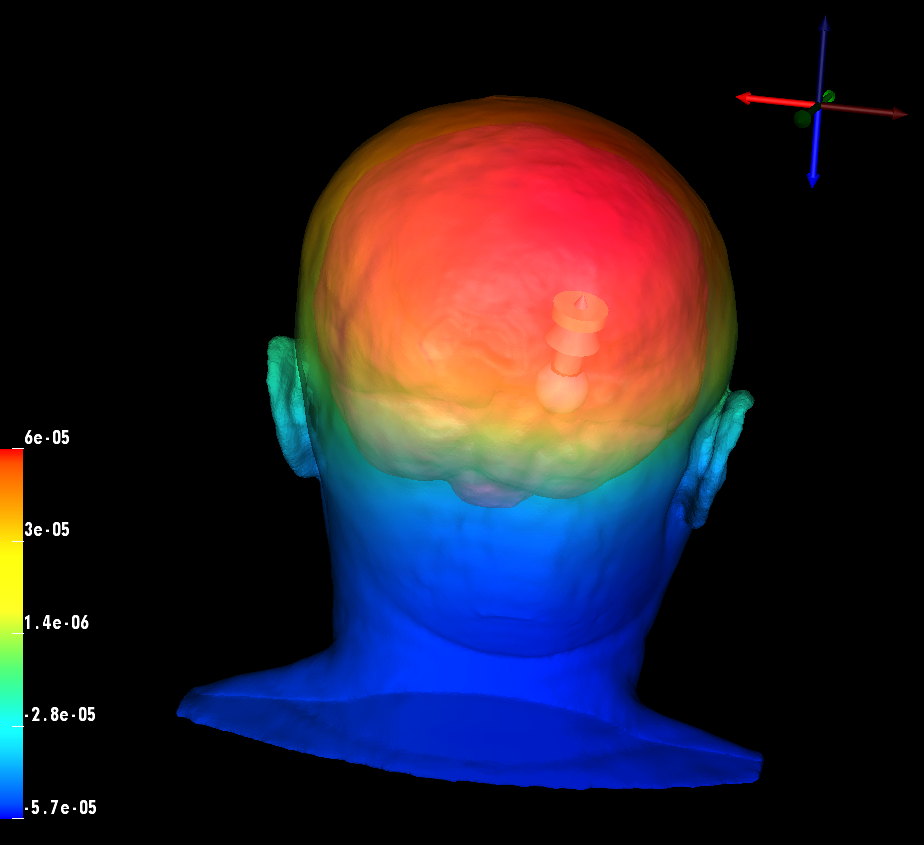
\includegraphics[width=.49\textwidth]{Figures/aniso_dipole_2}
\caption{Anisotropic forward problem solution with dipole source and data mapped onto the head surface and electrodes}
\label{fig:anisodip}
\end{center}
\end{figure}

\begin{figure}[H]
\begin{center}
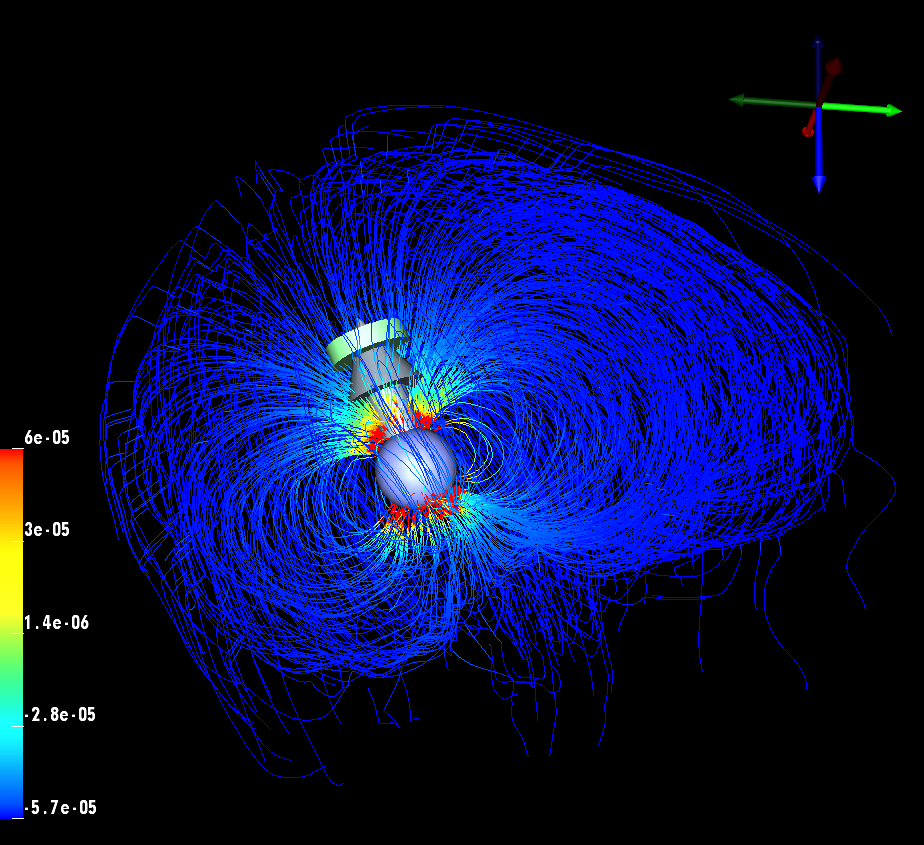
\includegraphics[width=.49\textwidth]{Figures/aniso_streamlines}
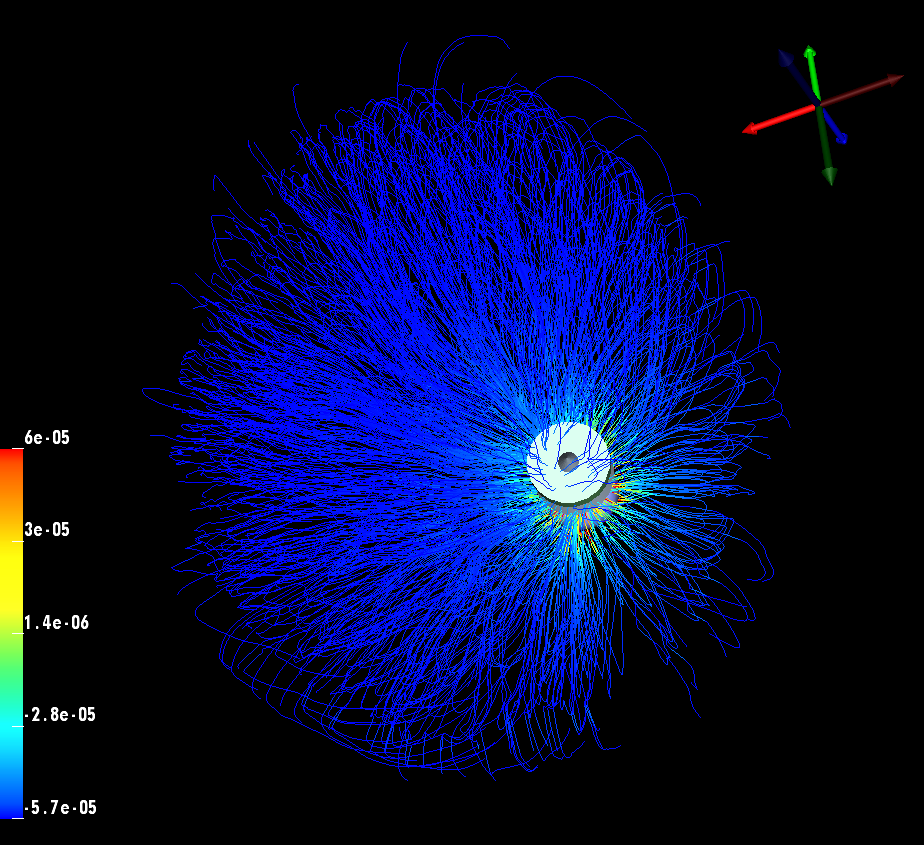
\includegraphics[width=.49\textwidth]{Figures/aniso_streamlines_top}
\caption{Anisotropic streamlines visualization with dipole source}
\label{fig:anisostream}
\end{center}
\end{figure}

\begin{figure}[H]
\begin{center}
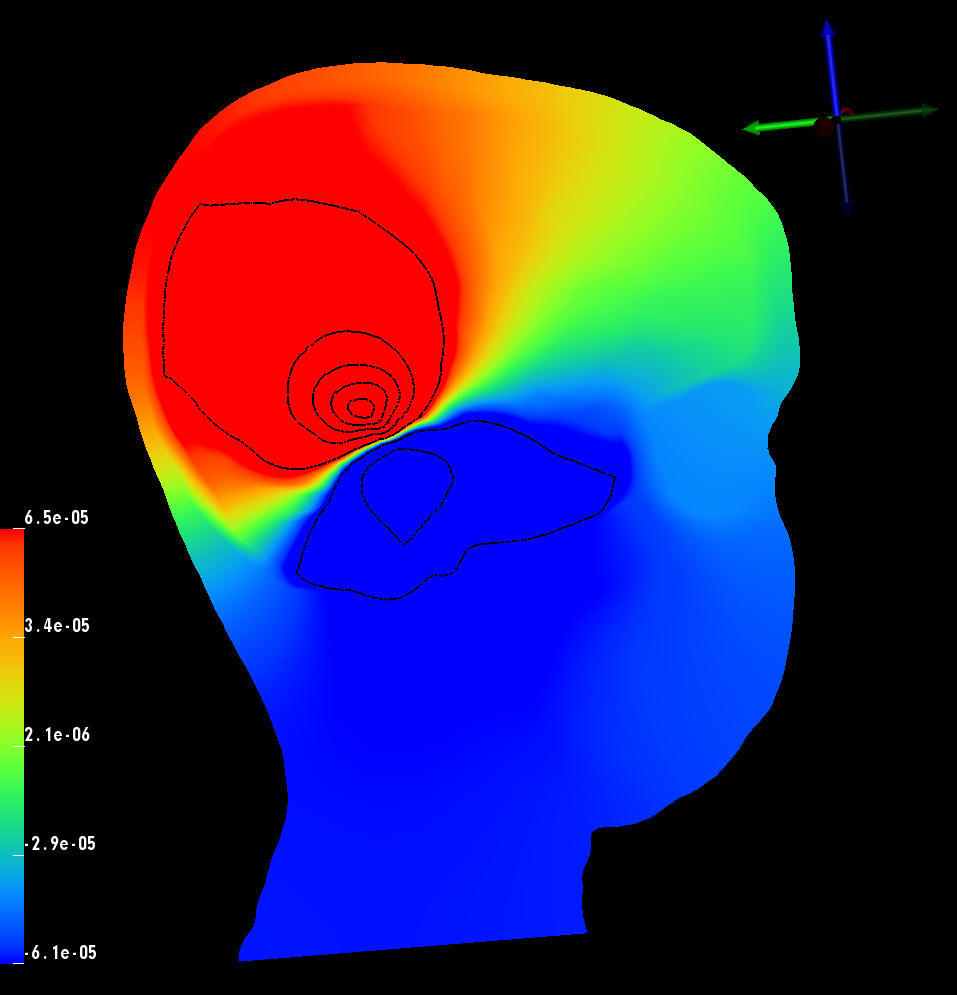
\includegraphics[width=.49\textwidth]{Figures/iso_isolines}
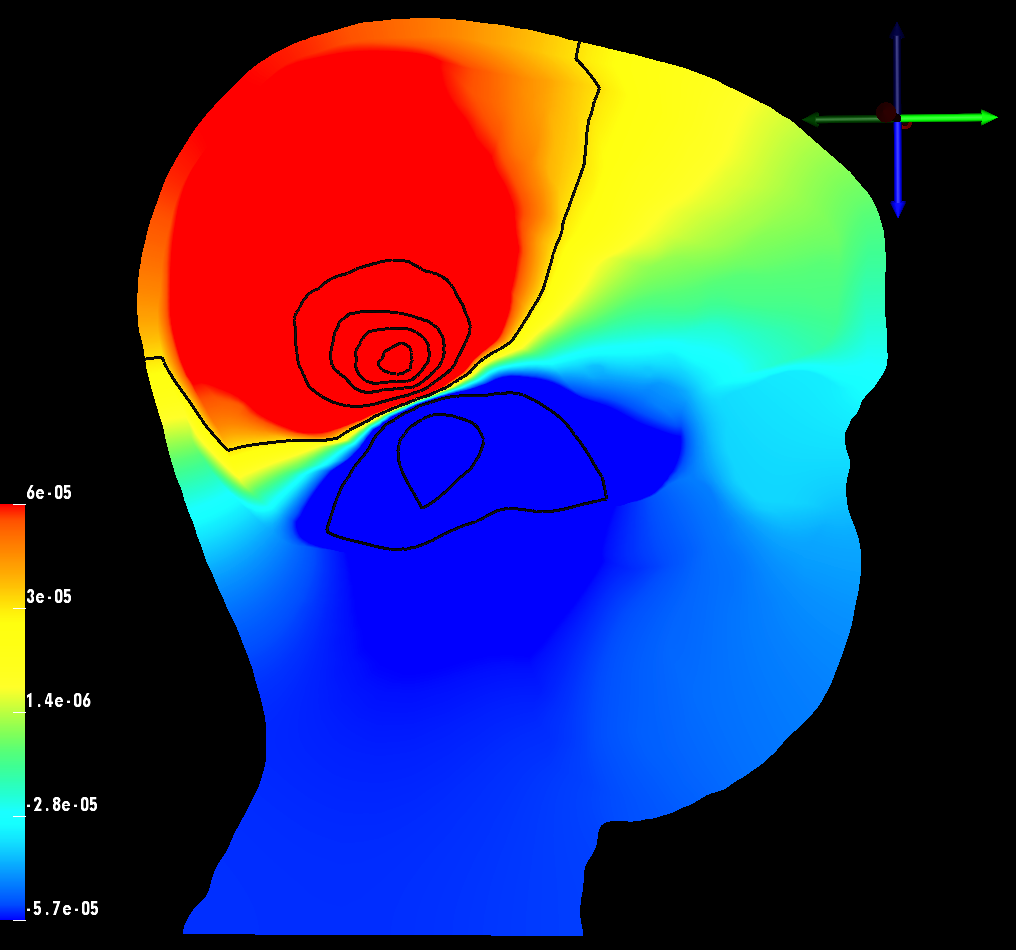
\includegraphics[width = .49\textwidth]{Figures/aniso_isolines}
\caption{Isolines comparison: isotropic white matter conductivity \textit{(left)}, anisotropic white matter conductivity \textit{(right)}}
\label{fig:isolines}
\end{center}
\end{figure}

\subsection{fMRI Visualization}

fMRI data was a novel imaging datatype for SCIRun. We successfully mapped and visualized the fMRI data onto the cortical surface with a rigid and manual registration to the mesh coordinate space. This mapping network allows for future use of fMRI data in simulations using the SCIRun software package.

\begin{figure}[H]
\begin{center}
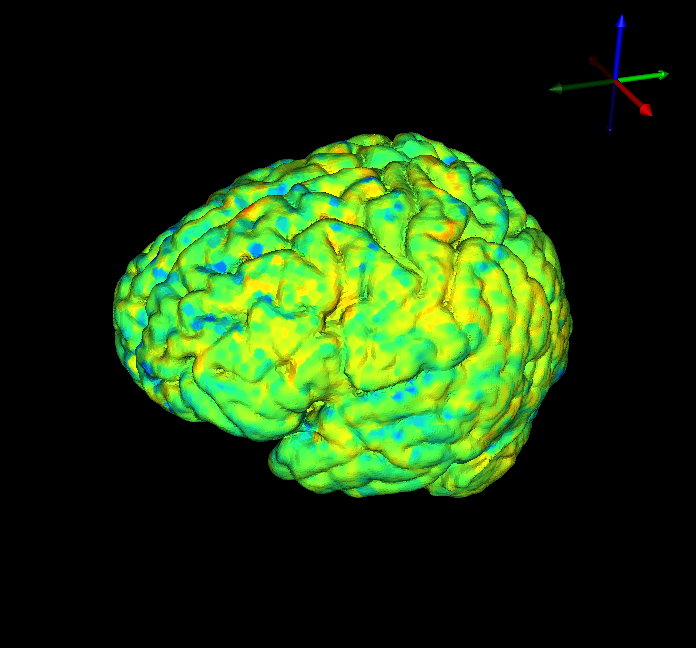
\includegraphics[width=.75\textwidth]{Figures/fmri_1}
\caption{fMRI data mapped onto cortical surface mesh}
\label{fig:fmrivis}
\end{center}
\end{figure}

\subsection{EEG Visualization}

When using EEG data, the particular application dictates if further processing, filtering, or cutting of the data is necessary. This EEG dataset, taken with 256 electrodes, contained electrodes that require further processing, specifically around the eyes, which was possibly due to the blinking or rolling of the subject's eyes. The bad leads will be fixed with further specific processing or trilinear interpolation.

\begin{figure}[H]
\begin{center}
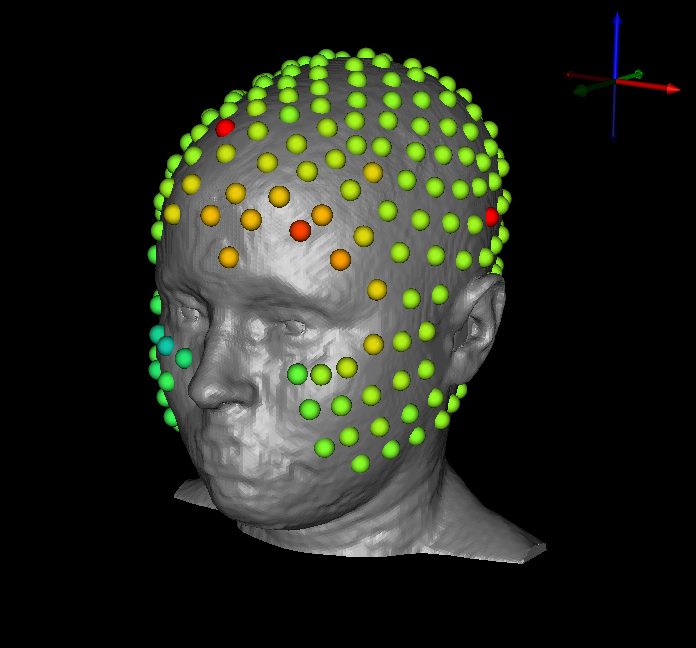
\includegraphics[width=.49\textwidth]{Figures/eeg_1}
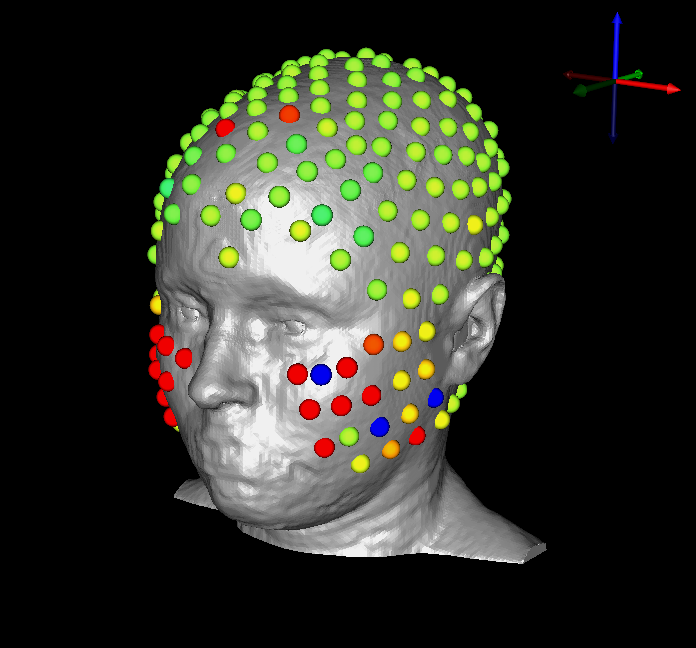
\includegraphics[width=.49\textwidth]{Figures/eeg_2}
\caption{EEG signal visualization with 256 electrodes. Examples of electrodes that require further processing for specific applications - shown in red.}
\label{fig:eegvis}
\end{center}
\end{figure}
The second EEG dataset, taken with 128 electrodes, still has electrodes that require further processing around the eyes. Since they electrodes don't go as far down the cheeks as the other dataset, we don't see as many electrodes that would need further processing. Although, there were time steps that did not register the data as well as others. 

\begin{figure}[H]
\begin{center}
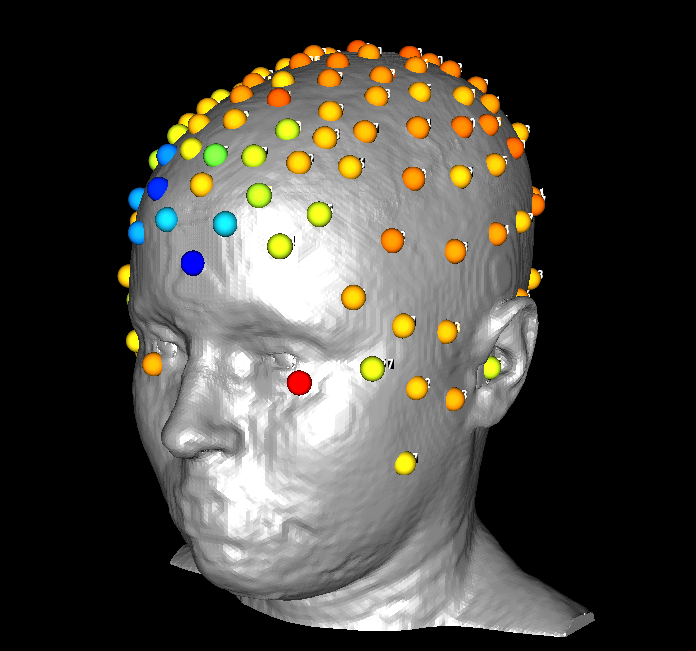
\includegraphics[width=.49\textwidth]{Figures/128_eeg_1}
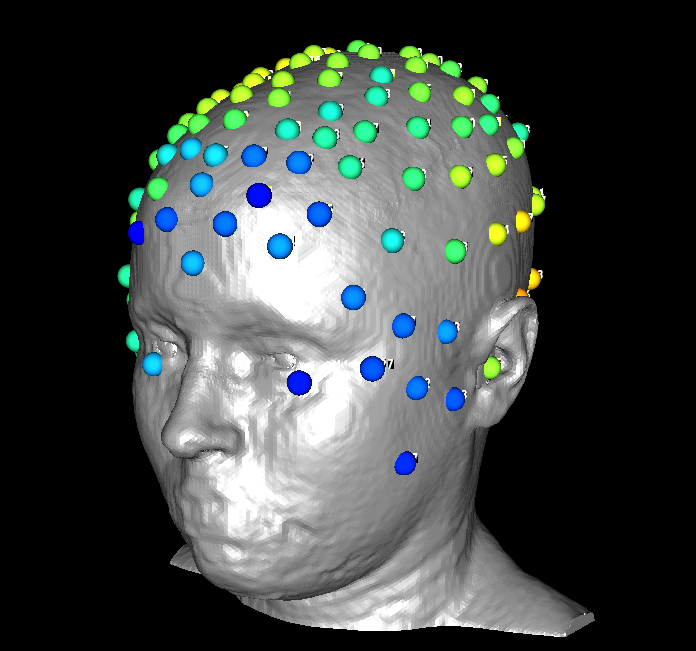
\includegraphics[width=.49\textwidth]{Figures/128_eeg_2}
\caption{EEG signal visualization with 128 electrodes. Examples of electrodes that require further processing for specific applications - shown in red.}
\label{fig:eegvis}
\end{center}
\end{figure}